% +--------------------------------------------------------------------+
% | Sample Chapter 3
% +--------------------------------------------------------------------+

\cleardoublepage

% +--------------------------------------------------------------------+
% | Replace "This is Chapter 3" below with the title of your chapter.
% | LaTeX will automatically number the chapters.                      
% +--------------------------------------------------------------------+

\chapter{Model Development}
\label{chp3}

Chapter \ref{chp3} will be dedicated to developing the various parameters that make up the NERMLAB such as the motor torque constant, \ac{back-emf}, inductance, and max voltage. Each section in Chapter \ref{chp3} will detail the process of how the various parameters were measured, calculated, and experimentally determined. Nomenclature for various constants and parameters are detailed in the table \ref{table2}.

% Table of motor lab constants
\begin{table}[ht]
\begin{center}
\caption{Motor parameters}
\begin{tabular}[c]{|c|c|}

\hline
\textbf{Parameter} & \textbf{Description}\\

\hline
V & Motor Voltage\\

\hline
\(k_t\) & Motor Torque Constant per Phase\\

\hline
\(k_T\) & Overall Motor Torque Constant\\

\hline
\(K_e\) & Back Electromotive Force Constant per Phase\\

\hline
\(K_{e,LL}\) & Line-Line Back Electromotive Force Constant\\

\hline
J & Mass Moment of Inertia\\

\hline
L & Motor Inductance\\

\hline
R & Motor Phase Resistance\\

\hline
\(R_{LL}\) & Motor Line-Line Resistance\\

\hline
\(\tau\) & Time Constant\\

\hline
T & Motor Torque\\
\hline
\(\omega_m\) & Motor Speed\\

\hline
\end{tabular}

\label{table2}
\end{center}
\end{table}

% end of table

\section{Motor Resistance}

\begin{figure}[H]%t=top, b=bottom, h=here
	\begin{center}
		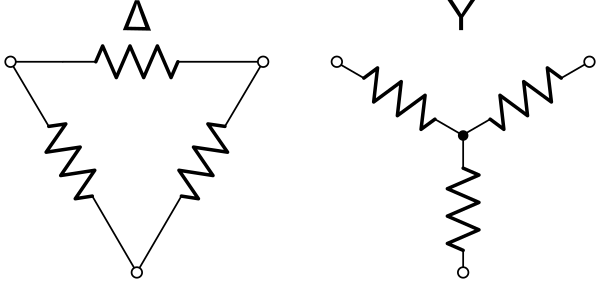
\includegraphics[height=1in]{figures/motor_winding.png}
		
		\caption[Motor Connection Configuration]{Motor Connection Configuration}
		
		\label{motor_configuration}
	\end{center}
\end{figure}

BLDC motors are typically connected in two wiring configurations, WYE (Y) or delta (\(\Delta \)) which can be seen in figure \ref{motor_configuration}. The RCTIMER GBM2804 utilizes the WYE (Y) configuration and will be analyzed as such. Due to the wiring of WYE systems, the neutral connection is typically unavailable for measurement on most motors. As a result it is common to measure resistance by a line-line reading. However in terms of motor control it is the phase resistance and not the line-line resistance that is of importance. Converting between the phase and line-line resistance is quite simple and can be done by dividing the line-line resistance by two (equation \ref{eq:3.1}).

\begin{equation} \label{eq:3.1}
R = \frac{R_{LL}}{2}
\end{equation}

\subsection{Procedure and Results}

In order to gather a good estimate for the phase resistance of the RCTIMER GBM2804 motor, the resistance was measured line-line across all 3 phases. Each set of motor leads were hooked up to a digital multimeter and the values were tabulated for each phase component in table \ref{table3}. An average was then calculated between the different line-line resistances to get the overall resistance of the motor.

\begin{table}[ht]
	\begin{center}
		\caption{Measured motor resistance}
		\begin{tabular}[c]{|c|c|c|}
			
			\hline
			\textbf{A-B} & \textbf{A-C} & \textbf{B-C}\\
			
			\hline
			9.870 \(\Omega\)  & 9.900  \(\Omega\) & 9.950 \(\Omega\) \\
			
			\hline
			& Average: & 9.91 \(\Omega\) \\
			
			\hline
			\end{tabular}
			
			\label{table3}
			\end{center}
			\end{table}

Using equation \ref{eq:3.1} it is then possible to find the overall phase resistance of the motor.

\begin{tcolorbox}[standard jigsaw,
	opacityback=0]
	\[R = 4.955 \approx 5 \Omega \]
	
\end{tcolorbox}

\section{Motor Torque Constant and Back EMF}
The motor torque constant (\(k_t\)) is a common parameter used in BLDC motors. It relates the armature current to the torque produced by a motor: \(T = k_T i \). Many methods exist to determine the torque constant, including relating the motor velocity constant \(k_v\) which is inversely related to the torque constant by \(k_T = \frac{1}{k_v} \), or by measuring the line-line back-emf voltage per phase (\(K_e\)). \(K_e\) is the peak value of the back-emf per angular velocity measured from line-neutral. However since line-neutral is typically unavailable on most BLDC motors, the back-emf constant is often represented as a line measurement, \(K_{e,LL}\). The overall torque constant can then be related to the line measurement back-emf voltage for sinusoidal type outputs by equation \ref{eq:3.2} or for trapezoidal outputs by equation \ref{eq:3.3}. \citep{5}. 

\begin{equation} \label{eq:3.2}
k_T = \frac{\sqrt{3}}{2} K_{e,LL}
\end{equation}

\begin{equation} \label{eq:3.3}
k_T = K_{e,LL}
\end{equation}

Because \(K_{e,LL}\) can be experimentally determined, it is possible to find the overall motor torque constant for a BLDC motor. One simply needs to measure the line-line sinusoidal or trapezoidal back-emf voltage at various speeds to get a good estimate of \(K_{e,LL}\). With equation \ref{eq:3.2} or \ref{eq:3.3}, \(k_T\) can then be determined.

\subsection{Procedure and Results}
In order to calculate the back-emf of the RCTIMER GBM2804 BLDC motor an experiment had to be set up to measure the voltage generated by the motor. Three pieces of equipment were needed: an oscilloscope, the Motorlab, and a torque transmission shaft. The torque transmission shaft was a 3D printed part\footnote{Appendix \ref{Appendix:Key2} figure \ref{torque_transmission_shaft_drawing}} that allowed the Motorlab to spin the RCTIMER GBM2804 at a constant speed to generate a back voltage. A line-line voltage (peak-peak) was then read from the leads of the RCTIMER GBM2804 by an oscilloscope\footnote{Appendix \ref{Appendix:Key1} figure \ref{back_emf_measurement}}. The data collected is tabulated in table \ref{table3}.

\begin{table}[ht]
\begin{center}
\caption{Measured back voltage }
\begin{tabular}[c]{|c|c|c|c|}

\hline
\textbf{Speed (RPM)} & \textbf{Speed \(\omega_m\) (rad/s)} & \textbf{Peak-Peak Voltage (V)} & \textbf{Peak Voltage (V)}\\

\hline
300  & 31.41  & 4.64 & 2.32\\

\hline
500 & 52.36 & 7.60 & 3.8\\

\hline
1000 & 104.72 & 15.1 & 7.55\\

\hline
1500 & 157.10 & 22.0 & 11.0\\

\hline
2000 & 209.44 & 30.0 & 15.0\\

\hline
\end{tabular}

\label{table3}
\end{center}
\end{table}

There is a fairly linear relationship between the peak voltage and speed. Due to this fact \(K_{e,LL}\) can be approximated from the slope of \(\frac{V}{\omega_m}\). The normal equation from the least-squares method was employed to find the best fit for the data in table \ref{table3}. Two matrices were constructed from the data, namely \(\matrva{V}\) and \(\matrva{\omega_m}\).

\begin{equation} \label{eq:3.4}
K_{e,LL} = (\matrva{\omega_m \omega_m^T})^{-1} \matrva{\omega_m V^T}
\end{equation} 

From equation \ref{eq:3.4}, the back-emf constant was found to be: 
\[K_{e,LL} = 0.0713 \quad \frac{V \cdot s}{rad} \]

To verify that \(K_{e,LL}\) was the best fit to that data, \(K_{e,LL}\) was plotted against the collected data in figure \ref{back_emf_plot}.

\begin{figure}[H]%t=top, b=bottom, h=here
	\begin{center}
		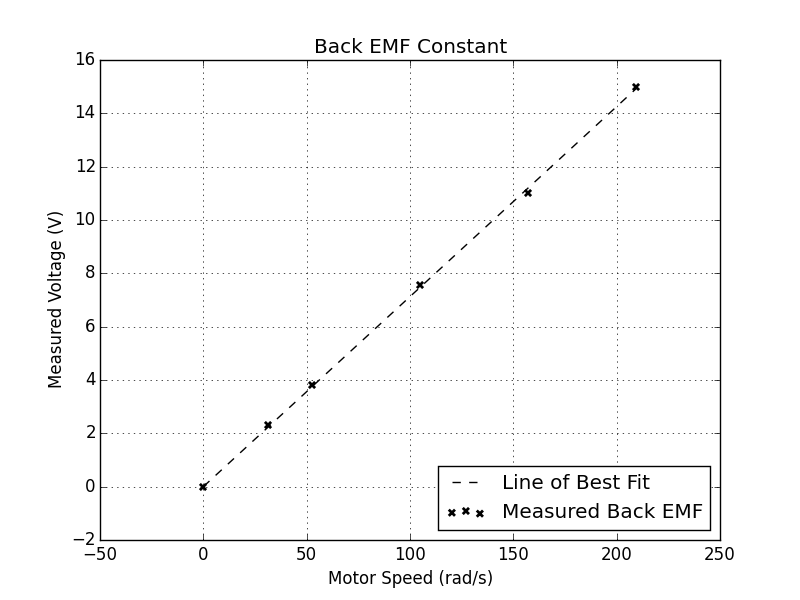
\includegraphics[height=3.8in]{figures/back_emf_plot.png}
		
		\caption[Measured Back EMF vs Speed]{Measured Back EMF vs Speed}
		
		\label{back_emf_plot}
	\end{center}
\end{figure}

Since the relationship between \(k_T\) and \(K_{e,LL}\) is known by equation \ref{eq:3.2} and \ref{eq:3.3}, \(k_T\) can now be calculated.
\begin{tcolorbox}[
    standard jigsaw,
    opacityback=0]
\[k_T = 0.0617 \approx 0.06 \quad \frac{N \cdot m}{s} \quad [Sinusoidal]\]
\[k_T =  0.0713 \approx 0.07 \quad  \frac{N \cdot m}{s} \quad [Trapezoidal]\]
\end{tcolorbox}

\newpage
\section{Mass Moment of Inertia Estimation}
Mass moment of inertia \(J\) is the equivalent to mass in a rotational system (commonly referred to as angular mass). More formally is it defined as \(J = \int r^2 dm\), where r is the distance to some mass from an axis of rotation.

The angular mass of the NERMLAB will be determined in two ways: experimentally determining \(J\) through software modeling, and approximating \(J\) through mathematical formulation. For both setups the mass of the rotating inertia had to be measured.

\subsection{Software Modeling of Mass Moment of Inertia}
\subsection{Mathematical Approximation of Mass Moment of Inertia}
To simplify the mathematical analysis of the mass moment of inertia calculation of the angular mass of the NERMLAB, an engineering assumption will be made that the angular mass is a rotating ring mass. This assumption is valid for the particular motor used in this thesis due to the fact that most of the mass is concentrated around the outside parameter of the motor. The outside ring mass of the motor contributes the most to the inertial load, so the mathematical formulation would result in the following equation:
\[J_z = \frac{m}{2}(r_1^2 + r_2^2) = mr_2^2(1-t+\frac{t^2}{2})\]

\begin{figure}[htb]%t=top, b=bottom, h=here
\begin{center}
    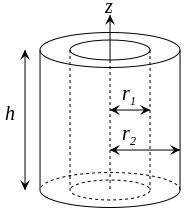
\includegraphics[height=1.5in]{figures/thick_walled_cylinder.png}

    \caption[Thick Walled Cylinder - Mass Moment of Inertia]{Thick Walled Cylinder (J)}

    \label{thick_walled_cylinder}
\end{center}
\end{figure}

\section{Motor Inductance}

\[L = R\tau\]